
\documentclass[12pt,a4paper, oneside]{extreport}

%%%%%%%%%% Математика %%%%%%%%%%
\usepackage{amsmath,amsfonts,amssymb,amsthm,mathtools}
% Показывать номера только у тех формул, на которые есть \eqref{} в тексте.
%\mathtoolsset{showonlyrefs=true}
%\usepackage{leqno} % Нумерация формул слева
%\usepackage{tipa} %Для формулки из логитов


\usepackage{hyphenat}

%%%%%%%%%% Шрифты %%%%%%%%
\usepackage[english, russian]{babel} % выбор языка для документа
\usepackage[utf8]{inputenc} % задание utf8 кодировки исходного tex файла
\usepackage[X2,T2A]{fontenc}        % кодировка

\usepackage{fontspec}         % пакет для подгрузки шрифтов
\setmainfont{Times New Roman}       % задаёт основной шрифт документа

\usepackage{unicode-math}      % пакет для установки математического шрифта
%\setmathfont{Asana-Math.otf}    % шрифт для математики

% Конкретный символ из конкретного шрифта
% \setmathfont[range=\int]{Neo Euler}


%%%%%%%%%% Работа с картинками %%%%%%%%%
\usepackage{graphicx}                  % Для вставки рисунков
\usepackage{graphics}
\graphicspath{{images/}{pictures/}}    % можно указать папки с картинками
\usepackage{wrapfig}                   % Обтекание рисунков и таблиц текстом


%%%%%%%%%% Работа с таблицами %%%%%%%%%%
\usepackage{tabularx}            % новые типы колонок
\usepackage{tabulary}            % и ещё новые типы колонок
\usepackage{array,delarray}      % Дополнительная работа с таблицами
\usepackage{longtable}           % Длинные таблицы
\usepackage{multirow}            % Слияние строк в таблице
\usepackage{float}               % возможность позиционировать объекты в нужном месте

\usepackage{booktabs}            % таблицы как в книгах

% Заповеди из документации к booktabs:
% 1. Будь проще! Глазам должно быть комфортно
% 2. Не используйте вертикальные линни
% 3. Не используйте двойные линии. Как правило, достаточно трёх горизонтальных линий
% 4. Единицы измерения - в шапку таблицы
% 5. Не сокращайте .1 вместо 0.1
% 6. Повторяющееся значение повторяйте, а не говорите "то же"
% 7. Есть сомнения? Выравнивай по левому краю!

%  вычисляемые колонки по tabularx
\newcolumntype{C}{>{\centering\arraybackslash}X}
\newcolumntype{L}{>{\raggedright\arraybackslash}X}
\newcolumntype{Y}{>{\arraybackslash}X}
\newcolumntype{Z}{>{\centering\arraybackslash}X}


%%%%%%%%%% Графика и рисование %%%%%%%%%%
\usepackage{tikz, pgfplots}      % язык для рисования графики из latex'a

%%%%%%%%%% Гиперссылки %%%%%%%%%%
\usepackage{xcolor}              % разные цвета

\usepackage{hyperref}
\hypersetup{
	unicode=true,           % позволяет использовать юникодные символы
	colorlinks=true,       	% true - цветные ссылки, false - ссылки в рамках
	urlcolor =blue,         % цвет ссылки на url
	linkcolor=black,        % внутренние ссылки
	citecolor=black,        % на библиографию
	breaklinks              % если ссылка не умещается в одну строку, разбивать ли ее на две части?
}


%%%%%%%%%% Другие приятные пакеты %%%%%%%%%
\usepackage{multicol}       % несколько колонок
\usepackage{verbatim}       % для многострочных комментариев
\usepackage{cmap} % для кодировки шрифтов в pdf

\usepackage{enumitem} % дополнительные плюшки для списков
%  например \begin{enumerate}[resume] позволяет продолжить нумерацию в новом списке

\usepackage{todonotes} % для вставки в документ заметок о том, что  осталось сделать
% \todo{Здесь надо коэффициенты исправить}
% \missingfigure{Здесь будет Последний день Помпеи}
% \listoftodos --- печатает все поставленные \todo'шки



%%%%%%%%%%%%%% ГОСТОВСКИЕ ПРИБАМБАСЫ %%%%%%%%%%%%%%%

%%% размер листа бумаги
\usepackage[paper=a4paper,top=15mm, bottom=15mm,left=35mm,right=10mm,includehead]{geometry}


\usepackage{setspace}
\setstretch{1.5}     % Межстрочный интервал
\setlength{\parindent}{1.25cm} % Красная строка.


%\flushbottom       % Эта команда заставляет LaTeX чуть растягивать строки, чтобы получить идеально прямоугольную страницу
\righthyphenmin=2  % Разрешение переноса двух и более символов
\widowpenalty=10000  % Наказание за вдовствующую строку (одна строка абзаца на этой странице, остальное --- на следующей)
\clubpenalty=10000  % Наказание за сиротствующую строку (омерзительно висящая одинокая строка в начале страницы)
\tolerance=1000     % Ещё какое-то наказание.


% Нумерация страниц сверху по центру
\usepackage{fancyhdr}
\pagestyle{fancy}
%\fancyhead{ } % clear all fields
%\fancyfoot{ } % clear all fields
\fancyhf{}
\fancyhead[R]{Касьянова Ксения (СМАР19): $k=1, r = 2$}
\fancyfoot[C]{\thepage}
% Чтобы не прорисовывалась черта!
\renewcommand{\headrulewidth}{0pt}


% Нумерация страниц с надписью "Глава"
\usepackage{etoolbox}
\patchcmd{\chapter}{\thispagestyle{plain}}{\thispagestyle{fancy}}{}{}


%%% Заголовки
\usepackage[indentfirst]{titlesec}{\raggedleft}
% Заголовки по левому краю
% опция identfirst устанавливает отступ в первом абзаце



% В Linux этот пакет сделан косячно. Исправляет это следующий непонятный кусок кода.
\makeatletter
\patchcmd{\ttlh@hang}{\parindent\z@}{\parindent\z@\leavevmode}{}{}
\patchcmd{\ttlh@hang}{\noindent}{}{}{}
\makeatother


% Редактирования Глав и названий
\titleformat{\chapter}
{\normalfont\large\bfseries}
{\thechapter }{0.5 em}{}

% Редактирование ненумеруемых глав chapter* (Введение и тп)
\titleformat{name=\chapter,numberless}
{\centering\normalfont\bfseries\large}{}{0.25em}{\normalfont}

% Убирает чеканутые отступы вверху страницы
\titlespacing{\chapter}{0pt}{-\baselineskip}{\baselineskip}

% Более низкие уровни
\titleformat{\section}{\bfseries}{\thesection}{0.5 em}{}
\titleformat{\subsection}{\bfseries}{\thesubsection}{0.5 em}{}

\titlespacing*{\section}{0 pt}{\baselineskip}{\baselineskip}
\titlespacing*{\subsection}{0 pt}{\baselineskip}{\baselineskip}


% Содержание. Команды ниже изменяют отступы и рисуют точечки!
\usepackage{titletoc}

\titlecontents{chapter}
[1em] %
{\normalsize}
{\contentslabel{1 em}}
{\hspace{-1 em}}
{\normalsize\titlerule*[10pt]{.}\contentspage}

\titlecontents{section}
[3 em] %
{\normalsize}
{\contentslabel{1.75 em}}
{\hspace{-1.75 em}}
{\normalsize\titlerule*[10pt]{.}\contentspage}

\titlecontents{subsection}
[6 em] %
{\normalsize}
{\contentslabel{3 em}}
{\hspace{-3 em}}
{\normalsize\titlerule*[10pt]{.}\contentspage}


% Правильные подписи под таблицей и рисунком
% Документация к пакету на русском языке!
\usepackage[tableposition=top, singlelinecheck=false]{caption}
\usepackage{subcaption}


\DeclareCaptionStyle{base}%
[justification=centering,indention=0pt]{}
\DeclareCaptionLabelFormat{gostfigure}{Рисунок #2}
\DeclareCaptionLabelFormat{gosttable}{Таблица #2}

\DeclareCaptionLabelSeparator{gost}{~---~}
\captionsetup{labelsep=gost}

\DeclareCaptionStyle{fig01}%
[margin=5mm,justification=centering]%
{margin={3em,3em}}
\captionsetup*[figure]{style=fig01,labelsep=gost,labelformat=gostfigure,format=hang}

\DeclareCaptionStyle{tab01}%
[margin=5mm,justification=centering]%
{margin={3em,3em}}
\captionsetup*[table]{style=tab01,labelsep=gost,labelformat=gosttable,format=hang}


% межстрочный отступ в таблице
\renewcommand{\arraystretch}{1.2}



% многостраничные таблицы под РОССИЙСКИЙ СТАНДАРТ
% ВНИМАНИЕ! Обязательно за CAPTION !
\usepackage{fr-longtable}



%Более гибкие спсики
\usepackage{enumitem}
% сообщаем окружению о том, что существует такая штук как нумерация русскими буквами.
\makeatletter
\AddEnumerateCounter{\asbuk}{\russian@alph}{щ}
\makeatother


%%% ГОСТОВСКИЕ СПИСКИ

% Первый тип списков. Большая буква.
\newlist{Enumerate}{enumerate}{1}

\setlist[Enumerate,1]{labelsep=0.5em,leftmargin=1.25em,labelwidth=1.25em,
	parsep=0em,itemsep=0em,topsep=0ex, before={\parskip=-1em},label=\arabic{Enumeratei}.}


% Второй тип списков. Маленькая буква.
\setlist[enumerate]{label=\arabic{enumi}),parsep=0em,itemsep=0em,topsep=0.75ex, before={\parskip=-1em}}


% Третий тип списков. Два уровня.
\newlist{twoenumerate}{enumerate}{2}
\setlist[twoenumerate,1]{itemsep=0mm,parsep=0em,topsep=0.75ex,, before={\parskip=-1em},label=\asbuk{twoenumeratei})}
\setlist[twoenumerate,2]{leftmargin=1.3em,itemsep=0mm,parsep=0em,topsep=0ex, before={\parskip=-1em},label=\arabic{twoenumerateii})}


% Четвёртый тип списков. Список с тире.
\setlist[itemize]{label=--,parsep=0em,itemsep=0em,topsep=0ex, before={\parskip=-1em},after={\parskip=-1em}}


%%% WARNING WARNING WARNIN!
%%% Если в списке предложения, то должна по госту стоять точка после цифры => команда Enumerate! Если идет перечень маленьких фактов, не обособляемых предложений то после цифры идет скобка ")" => команда enumerate! Если перечень при этом ещё и двууровневый, то twoenumerate.




%%%%%%%%%% Список литературы %%%%%%%%%%

%\usepackage[%
%backend=biber, %подключение пакета biber (тоже нужен)
%bibstyle=gost-numeric, %подключение одного из четырех главных стилей biblatex-gost
%sorting=ntvy, %тип сортировки в библиографии
%]{biblatex}

\usepackage[backend=biber,style=gost-numeric, maxbibnames=9,maxcitenames=2,uniquelist=false, babel=other]{biblatex}



% Справка по 4 главным стилям для ленивых:
% gost-inline  ссылки внутри теста в круглых скобках
% gost-footnote подстрочные ссылки
% gost-numeric затекстовые ссылки
% gost-authoryear тоже затекстовые ссылки, но немного другие

% Подробнее смотри страницу 4 документации. Она на русском.

% Ещё немного настроек
\DeclareFieldFormat{postnote}{#1} %убирает с. и p.
\renewcommand*{\mkgostheading}[1]{#1} % только лишь убираем курсив с авторов


\addbibresource{diploma11.bib} % сюда нужно вписать свой bib-файлик.



% Этот кусок кода выносит русские источники на первое место. Костыль описали авторы пакета в руководстве к нему. Подробнее смотри:
% https://github.com/odomanov/biblatex-gost/wiki/Как-сделать%2C-чтобы-русскоязычные-источники-предшествовали-остальным
\DeclareSourcemap{
	\maps[datatype=bibtex]{
		\map{
			\step[fieldsource=langid, match=russian, final]
			\step[fieldset=presort, fieldvalue={a}]
		}
		\map{
			\step[fieldsource=langid, notmatch=russian, final]
			\step[fieldset=presort, fieldvalue={z}]
		}
	}
}

\DefineBibliographyStrings{english}{%
	pages = {P\adddot},
	number = {№},
}



\begin{document} % Начала документа



%%%%%%%%%%%%%%%%%%%% ВВЕДЕНИЕ %%%%%%%%%%%%%%%%%%%%%%%%%%%%%%%%%%%%
\section*{I часть. LIFE INSURANCE}


\begin{figure}
	\centering
	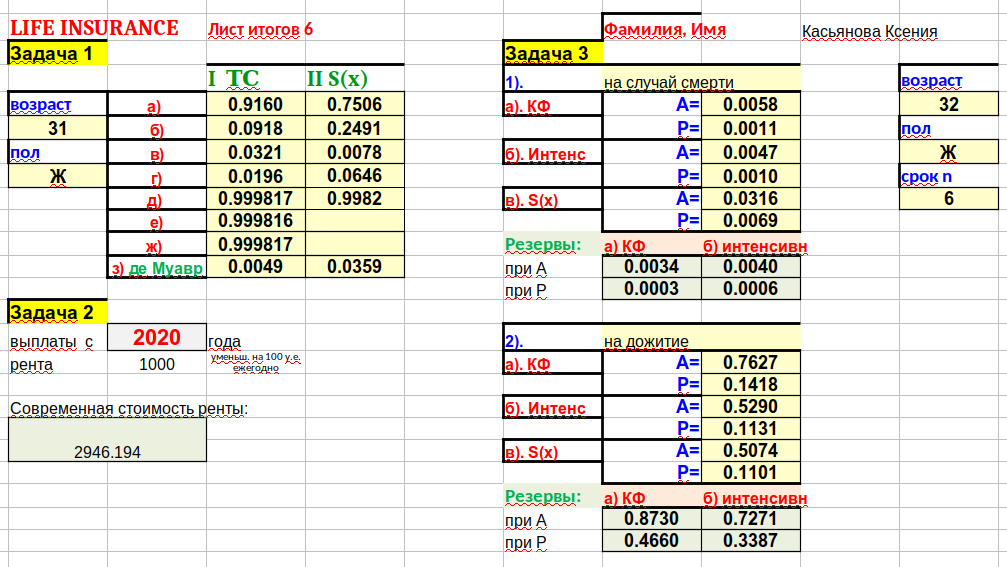
\includegraphics[width=1\linewidth]{screenshot005}
	\label{fig:screenshot005}
\end{figure}




\subsection*{Задача 1}

Найти вероятности  для 31-летнего страхователя:

I. по таблице смертности жителей г. Москвы за 2016 г. для  
страхователя – женщины:

II. для функции дожития вида:  $s(x) = \sqrt{1-\frac{x}{102}},  
0 \leq x \leq 102 $

III.  для интенсивности  смертности вида: $\mu_x = 0.002x, x\geq 0$



а) дожить, по крайней мере, до 62 лет

I. $_{31}p_{31} = \dfrac{l_{62}}{l_{31}} = \dfrac{90087}{98351} = 0.91597$  

II. $_{31}p_{31} = \dfrac{s(62)}{s(31)} = \frac{\sqrt{1-\frac{62}{102}}}{\sqrt{1-\frac{31}{102}}} = 0.75058$  


III. $_{31}p_{31} =  \exp(-\int_{31}^{62} 0.002u  du  )  = \exp(-2.883)  = 0.05596$  
 

б) умереть до достижения возраста 52 лет;

I. $_{21}q_{31} = \frac{l_{31} - l_{62}}{l_{31}} = \frac{98351-90087}{98351} = 0.09181$  

II. $_{21}q_{31} = \dfrac{s(31) - s(62)}{s(31)} = \frac{\sqrt{1-\frac{31}{102}}-\sqrt{1-\frac{62}{102}}}{\sqrt{1-\frac{31}{102}}} = 0.24941$  


III. $_{21}q_{31} = 1 - \exp(-\int_{31}^{52} 0.002u du  )  = 1 -  \exp(-1.743)  = 0.825   $  
 


в) умереть в возрасте 44 лет;

I. $_{13|}q_{31} = \dfrac{l_{44} - l_{45}}{l_{31}} = \dfrac{96668-96479}{98351} = 0.00192$  

II. $_{13|}q_{31} = \dfrac{s(44) - s(45)}{s(31)} = \frac{\sqrt{1-\frac{44}{102}}-\sqrt{1-\frac{45}{102}}}{\sqrt{1-\frac{31}{102}}} = 0.00782$  

III. $_{13|}q_{31} = _{13}p_x -  _{14}p_x  =  \exp(-\int_{31}^{44} 0.002u  du  ) - \exp(-\int_{31}^{45} 0.002u  du  )  = \exp(-0.975)  - \exp(-1.064) = 0.03211 $  


г) умереть в возрасте от 44 до 52 лет;

I. $_{13|8}q_{31} = \dfrac{l_{44} - l_{52}}{l_{31}} = \dfrac{96668-94737}{98351} = 0.01963$  

II. $_{13|8}q_{31} = \dfrac{s(44) - s(52)}{s(31)} = \frac{\sqrt{1-\frac{44}{102}}-\sqrt{1-\frac{52}{102}}}{\sqrt{1-\frac{31}{102}}} = 0.06464$  


III.  $_{13|8}q_{31} = _{13}p_x -  _{21}p_x  =  \exp(-\int_{31}^{44} 0.002u  du  ) - \exp(-\int_{31}^{52} 0.002u  du  )  = \exp(-0.975)  - \exp(-1.743) = 0.2022 $  



д-ж) прожить ещё 3 месяца 

I. - в предположении о линейности функции дожития;

 $_{0.25}p_{31} = 1 - _{0.25}q_{31} = 1 - 0.25 q_{31} = 1 - 0.25 * 0.000732  = 0.999817$  

- в предположении о постоянстве силы смертности;

 $_{0.25}p_{31} =  p_{31}^{0.25}  = (1-0.000732)^{0.25} = 0.999816$  


- в предположении гипотезы Балдуччи;

$_{0.25}p_{31} =  \dfrac{p_{31}}{p_{31} + 0.25 q_{31} }   =  \frac{1-0.000732}{1-0.000732 + 0.25 * 0.000732 } = 0.999817$  


II.  $_{0.25}p_{31} = \dfrac{s(31.25)}{s(31)} = \frac{\sqrt{1-\frac{31.25}{102}}}{\sqrt{1-\frac{31}{102}}} = 0.99824 $  




III. $_{0.25}p_{31} =  \exp(-\int_{31}^{31.25} 0.002u  du  )  = \exp(-0.0156)  = 0.98452$  




з) средняя округленная продолжительность
оставшейся жизни по таблицам смертности: $ e_{31}  = [T_{31}] = [50.50] = 50  $;
и средняя полная продолжительность
оставшейся жизни по функции дожития:  $\mathring{e}_{31} = E(T_{31}) = \frac{1}{s(31)} \int_{31}^{102} \sqrt{1-\frac{u}{102}}du = 1.1986 * 39.491 = 47.334$


и) умереть в течение последующих 5
лет

по де Муавру с предельным возрастом 100 лет: $_5q_{31}=\dfrac{s(31)-s(36)}{s(31)} = (\frac{100-31}{100} -\frac{100-36}{100})/ \frac{100-31}{100}  = 0.07246$

I. $_5q_{31}=\dfrac{l_{31}-l_{36}}{l_{31}} = \dfrac{98351-97868}{98351} = 0.00491 $

II. $_5q_{31}=\dfrac{s(31)-s(36)}{s(31)} =  0.03585 $

III. $_{5}q_{31} = 1 - \exp(-\int_{31}^{36} 0.002u du  )  = 1 -  \exp(-0.335)  = 0.28466   $  


к) кривая смертей $f(x)$, интенсивность смертности $\mu_x$, функция дожития $s(x)$

I. $f(x) = - s'(x) = - \dfrac{d}{dx}(\sqrt{1-\frac{x}{102}}) =  \frac{1}{204 \sqrt{1-\frac{x}{102}} }$

$\mu_{x} = \frac{f(x)}{s(x)} =  \frac{1}{204 (1-\frac{x}{102}) }  $


II. $s(x) = \exp(- 0.001 x^2) $

$f(x) = - s'(x)=  0.002  \exp(- 0.001 x^2)  x  $

\subsection*{Задача 2}
Эффективная
годовая процентная ставка $i_1 = 7 \%$  в течение первых 10 лет, $i_2 =4 \%$. 
В 2015 году покупается  8-летняя финансовая рента с выплатами
каждый год, начиная с 2020-го года (ровно через 5 лет), в первый год
выплат - 1000 у.е., \textit{уменьшающуюся} ежегодно на 100 у.е.

$\nu_1 =  0.9346, \nu_2= 0.9615$

$a_{\bar{5}|@i_1} = \frac{1-0.9346^5}{0.07}=4.099$

$(Ia)_{\bar{5}|@i_1} = \frac{4.099}{1-0.9346}-\frac{5*0.9346^5}{0.07}=11.743$

$(Da)_{\bar{5}|@i_1} = \frac{(5*0.07-1)*4.099}{0.07}+\frac{5*0.9346^5}{0.07}=12.87$


$a_{\bar{3}|@i_2} = \frac{1-0.9615^3}{0.04}=2.778$

$(Ia)_{\bar{3}|@i_2} = \frac{2.778}{1-0.9615}-\frac{3*0.9615^3}{0.04}=5.489$


$(Da)_{\bar{3}|@i_2} = \frac{(3*0.04-1)*2.778}{0.04}+\frac{3*0.9615^3}{0.04}=5.551$


а) Стоимость в момент заключения договора: 

- через возрастающую ренту 

$A = (1100 * a_{\bar{5}|@i_1} - 100 * (Ia)_{\bar{5}|@i_1}     +  600 * a_{\bar{3}|@i_2} * \nu_1^5   - 100 * (Ia)_{\bar{3}|@i_2}* \nu_1^5   )*\nu_1^5 = 
     (1100 * 4.099 - 100 * 11.743     +  600 * 2.778 * 0.9346^5   - 100 * 5.489* 0.9346^5   )*0.9346^5   = 2946.194$  

- через убывающую ренту

$A = (500 * a_{\bar{5}|@i_1} + 100 * (Da)_{\bar{5}|@i_1}     +  200 * a_{\bar{3}|@i_2} * \nu_1^5   + 100 * (Da)_{\bar{3}|@i_2}* \nu_1^5   )*\nu_1^5 = 
      (500 * 4.099 + 100 * 12.87     +  200 * 2.778 * 0.9346^5   + 100 * 5.551* 0.9346^5   )*0.9346^5 = 2943.888 $  


Стоимость, накопленная  к концу платежного периода: 

- через возрастающую ренту 

$S = (1100 * a_{\bar{5}|@i_1}*(1+i_1)^5 - 100 * (Ia)_{\bar{5}|@i_1} *(1+i_1)^5     +  600 * a_{\bar{3}|@i_2}     - 100 * (Ia)_{\bar{3}|@i_2}   )*(1+i_2)^3  
= (1100 * 4.099*1.07^5 - 100 * 11.743 * 1.07^5     +  600 * 2.778     - 100 * 5.489   )*1.04^3 = 6518.417 $
  


- через убывающую ренту.

$S = (500 * a_{\bar{5}|@i_1} *(1+i_1)^5 + 100 * (Da)_{\bar{5}|@i_1} *(1+i_1)^5    +  200 * a_{\bar{3}|@i_2}    + 100 * (Da)_{\bar{3}|@i_2}   )*(1+i_2)^3  = (500 * 4.099 *1.07^5 + 100 * 12.87 *1.07^5    +  200 * 2.778    + 100 * 5.551  )*1.04^3 = 6513.316$  



б) Премии, которые  должен внести страхователь, если он желает
оплатить договор двумя платежами:


$a_{\bar{1}|@i_1} = \frac{1-0.9346}{0.07}=0.934$

$(Ia)_{\bar{1}|@i_1} = \frac{0.934}{1-0.9346}-\frac{0.9346}{0.07}=0.9299$

$a_{\bar{4}|@i_1} = \frac{1-0.9346^4}{0.07}=3.386$

$(Ia)_{\bar{4}|@i_1} = \frac{3.386}{1-0.9346}-\frac{4*0.9346^4}{0.07}=8.176$

$a_{\bar{3}|@i_2} = \frac{1-0.9615^3}{0.04}=2.778$

$(Ia)_{\bar{3}|@i_2} = \frac{2.778}{1-0.9615}-\frac{3*0.9615^3}{0.04}=5.489$


- в момент заключения договора (первые 4 выплаты ренты);

$A_1 = (1100 * a_{\bar{4}|@i_1} - 100 * (Ia)_{\bar{4}|@i_1}  )*\nu_1^5 = (1100 * 3.386 - 100 * 8.176  )*0.9346^5
 =2072.879
 $  

- в момент начала выплат (последние четыре выплаты).

$A = (700 * a_{\bar{1}|@i_1} - 100 * (Ia)_{\bar{1}|@i_1}     +  600 * a_{\bar{3}|@i_2} * \nu_1   - 100 * (Ia)_{\bar{3}|@i_2}* \nu_1  )*\nu_1^5 = (700 * 0.934 - 100 * 0.9299     +  600 * 2.778 * 0.9346   - 100 * 5.489* 0.9346  )*0.9346^5 = 1144.896
$  




\subsection*{Задача 3}

Найти и сравнить единовременную (A) и ежегодную (P) премии по договорам
страхования для 32-летнего страхователя-женщины на сумму 20000 у.е. Найти величину страхового резерва на конец 3-го страхового года  $_3V_{  \overset{1}{x} : \bar{6}|@\delta_1}$  - 
для  стандартной процентной ставки  и  $_3V_{  \overset{1}{x} : \bar{6}|@\delta_2}$ - для процентной ставки, 
соответствующей интенсивности процентов $\delta=10,5\%$ .


1) на случай смерти на срок 6 лет (с выплатой в конце года смерти);

2) на дожитие на срок 6 лет;

3) смешанного страхования на срок 6 лет (с выплатой в конце года смерти);

а) для коммутационных функций для эффективной годовой процентной ставки $i=4,5\%$, представленной в таблице смертности.

1) с единовременной уплатой взносов

 $ A_{  \overset{1}{32} : \bar{6}|} = \frac{M_{32}-M_{38}}{D_{32}} = \frac{3227.84-3088.94}{24029.21} = 0.00578$

$_3V_{  \overset{1}{32} : \bar{6}|@\delta_1}^A = \frac{M_{35}-M_{38}}{D_{35}} = \frac{3161.01-3088.94}{20992.4360} = 0.00343  $


с ежегодной уплатой взносов

 $ P_{ \overset{1}{32} : \bar{6}|} = \frac{M_{32}-M_{38}}{N_{32}-N_{38}} = \frac{3227.84 -3088.94}{483054.06- 353850.19} = 0.00108$

$_3V_{  \overset{1}{32} : \bar{6}|@\delta_1}^P =  \frac{M_{35}-M_{38}}{D_{35}}  -  \frac{M_{32}-M_{38}}{N_{32}-N_{38}} * \frac{N_{35}-N_{38}}{D_{35}}  = 0.00343  -  \frac{3227.84-3088.94}{483054.06-353850.19} * \frac{414085.23-353850.19}{20992.4360}  =  0.000348$



2) с единовременной уплатой взносов

$ A_{32:  \overset{1}{\bar{6}}|} = \frac{D_{38}}{D_{32}} = 
\frac{18326.51}{24029.21} = 0.76268$

$_3V_{  32:  \overset{1}{\bar{6}}|@\delta_1}^A = \frac{D_{38}}{D_{35}} =  \frac{18326.51}{20992.43} = 0.873  $

с ежегодной уплатой взносов


 $ P_{ x:  \overset{1}{\bar{6}}|} = \frac{D_{38}}{N_{32}-N_{38}}= \frac{18326.51}{483054.06 - 353850.19}= 0.14184$

$_3V_{ 32:  \overset{1}{\bar{6}}|@\delta_1}^P = \frac{D_{38}}{D_{35}}  - \frac{D_{38}}{N_{32}-N_{38}}  * \frac{N_{35}-N_{38}}{D_{35}}  =   0.873   - \frac{18326.51}{483054.06-353850.19}  * \frac{414085.23-353850.19}{20992.43} = 0.466 $




3) с единовременной уплатой взносов 

$ A_{32: \bar{6}|} = A_{  \overset{1}{32} : \bar{6}|} + A_{32:  \overset{1}{\bar{6}}|} = 0.00578 + 0.76268 = 0.76846$


$_3V_{ 32: \bar{6}|@\delta_1}^A =  _3V_{  \overset{1}{32} : \bar{6}|@\delta_1}^A + _3V_{  32:  \overset{1}{\bar{6}}|@\delta_1}^A  =  0.00343 + 0.76268 =0.76611 $


с ежегодной уплатой взносов

$ P_{ 32:  \bar{6}| } = P_{ \overset{32}{x} : \bar{6}|} +  P_{ x:  \overset{1}{\bar{6}}|}  = 0.00108 + 0.14184 = 0.14292$

$_3V_{ 32: \bar{6}|@\delta_1}^P = _3V_{ 32: \bar{6}|@\delta_1}^A -
 \frac{D_{38}+M_{32}-M_{38}}{N_{32}-N_{38}}  * \frac{N_{35}-N_{38}}{D_{35}} = 0.76611   - \frac{18326.51+ 3227.84 - 3088.94}{483054.06-353850.19}  * \frac{414085.23-353850.19}{20992.43} = 0.35603
$


б) при интенсивности процентов $\delta=10,5\%$.

$\nu=\exp{-0.105} = 0.90032 $

1) с единовременной уплатой взносов

$ A_{  \overset{1}{32} : \bar{6}|} = \frac{\nu d_{32} + ... \nu^6*d_{37}}{l_{32}} = 0.00466$


$_3V_{  \overset{1}{32} : \bar{6}|@\delta_2}^A = A_{  \overset{1}{35} : \bar{3}|} = 0.00404 $

с ежегодной уплатой взносов

$ P_{ \overset{1}{32} : \bar{6}|} = \frac{\nu d_{32} + ... \nu^6*d_{37}}{l_{32} + ... \nu^5*d_{37}} = 0.000996$

$_3V_{  \overset{1}{32} : \bar{6}|@\delta_2} = _3V_{  \overset{1}{32} : \bar{6}}^A -  P_{ \overset{1}{32} : \bar{6}|} * \ddot{a}_{  \overset{1}{35} : \bar{3}} = 0.00404 -  0.000996 * 3.43497 = 0.00062 $


2) с единовременной уплатой взносов

$ A_{32:  \overset{1}{\bar{6}}|} = \nu^6 \frac{l_{38}}{l_{32}} = 0.52897$

$_3V_{32:  \overset{1}{\bar{6}}|@\delta_2}^A = A_{35:  \overset{1}{\bar{3}}|} = 0.72705$

с ежегодной уплатой взносов


$ P_{ x:  \overset{1}{\bar{6}}|} = \frac{\nu^6l_{38}}{l_{32} + ... \nu^5*d_{37}}= 0.11306$


$_3V_{  32:  \overset{1}{\bar{6}}|@\delta_2}^P = A_{35:  \overset{1}{\bar{3}}|} - P_{ x:  \overset{1}{\bar{6}}|}*\ddot{a}_{  \overset{1}{35} : \bar{3}} =   0.72705  -  0.11306 * 3.43497  = 0.338692$



3) с единовременной уплатой взносов 

$ A_{32: \bar{6}|} = A_{  \overset{1}{32} : \bar{6}|} + A_{32:  \overset{1}{\bar{6}}|} = 0.00466 + 0.52897 = 0.53363$


$_3V_{ 32: \bar{6}|@\delta_2}^A = A_{  \overset{1}{35} : \bar{3}|} =  0.00404 + 0.72705 =  0.73109$

с ежегодной уплатой взносов

$ P_{ 32:  \bar{6}| } = P_{ \overset{32}{x} : \bar{6}|} +  P_{ x:  \overset{1}{\bar{6}}|}  = 0.000996 + 0.11306 = 0.11405$


$_3V_{ 32: \bar{6}|@\delta_2}^P = A_{  \overset{1}{35} : \bar{3}|} - P_{ 32:  \bar{6}| } * \ddot{a}_{  \overset{1}{35} : \bar{3}} =  0.73109 -  0.11405 * 3.43497 = 0.33933 $




в) с использованием функции дожития вида:
$S(x) = \sqrt{1-\frac{x}{100}}, 0 \leq x \leq 100$ 
при эффективной учетной ставке $d=10\%$.

$\nu  = 1-d = 0.9$

$d_x = (s(x) - s(x+1))/ s(x) * l_0$

$l_x = s(x) * l_0$


1) с единовременной уплатой взносов

$ A_{  \overset{1}{32} : \bar{6}|} = \frac{\nu d_{32} + ... \nu^6*d_{37}}{l_{32}} = 0.031649$


с ежегодной уплатой взносов

$ P_{ \overset{1}{32} : \bar{6}|} = \frac{\nu d_{32} + ... \nu^6*d_{37}}{l_{32} + ... \nu^5*d_{37}} = 0.006866$



2) с единовременной уплатой взносов

$ A_{32:  \overset{1}{\bar{6}}|} = \nu^6 \frac{l_{38}}{l_{32}} = 0.50745$

с ежегодной уплатой взносов


$ P_{ x:  \overset{1}{\bar{6}}|} = \frac{\nu^6l_{38}}{l_{32} + ... \nu^5*d_{37}}= 0.110101$



3) с единовременной уплатой взносов 

$ A_{32: \bar{6}|} = A_{  \overset{1}{32} : \bar{6}|} + A_{32:  \overset{1}{\bar{6}}|} = 0.00466 + 0.52897 = 0.539103$


с ежегодной уплатой взносов

$ P_{ 32:  \bar{6}| } = P_{ \overset{32}{x} : \bar{6}|} +  P_{ x:  \overset{1}{\bar{6}}|}  = 0.000996 + 0.11306 = 0.116968$
















%%%%%%%%%%% Список литературы	%%%%%%%%%%%

%%%%%%%%%%%%%%%%%%%% Приложения %%%%%%%%%%%%%%%%%%%%

\appendix
\renewcommand{\thechapter}{\Asbuk{chapter}}

%%%%%%%%%% titlesec для приложений
\titleformat{\chapter}
 {\normalfont\bfseries\large}{\chaptertitlename~\thechapter}{0.25em}{\normalfont}



\end{document}
